\chapter{Systemmodelle}


\section{Interaktionsverlauf}

	\begin{longtable}{|p{0.25\textwidth}|p{0.75\textwidth}|}
    \hline
    main menu & Das ist die erste Ansicht, die der Nutzer bekommt. Von hier aus erreicht er alle Bereiche des Programms.\\
    \hline
    creative & Von hier aus startet der Nutzer ein neues Spiel, mit einem einfachem Standardknoten, lädt einen Speicherstand oder startet das erstellen von neuen Herausforderungen (challenges).\\
    \hline
    challenge & Eine Übersicht, der vorhandenen Herausforderungen. Der Nutzer kann nach verschieden Kriterien suchen und sortieren lassen und in einer Vorschau weitere Informationen betrachten.\\
    \hline
    settings & Einstellungen an Grafik, Ton und Steuerung. Außerdem kann die persönliche Farbpalette angepasst werden.\\
    \hline
    credits & Zeigt Infos über die Mitwirkenden an dem Programm und über das Programm selber.\\
    \hline
    
   \end{longtable}
   
   ~\\
    
	\begin{figure}[h]
		\centering
	 	\includesvg[width = 0.95\textwidth]{menu}
	 	\caption{Hauptmenüeinträge}
	\end{figure}
	
	\clearpage
	~\\
	
	Im Spiel kann der Nutzer auch die {\color{red} Einstellungen} erreichen. Die Menüeinträge in den unterschiedlichen Spielmodi können variieren.
		
	\begin{longtable}{|p{0.25\textwidth}|p{0.75\textwidth}|}
	
	\hline
	settings & Genau wie aus dem Hauptmenü.\\
	\hline
	save & Speichert den aktuellen Spielstand.\\
	\hline
	quit & Beendet das laufende Spiel. \\
	\hline
	render options & Bietet dem Nutzer verschiedene Möglichkeiten seinen Knoten zu rendern und zu exportieren.\\
	\hline
	
	\end{longtable}
	
	\begin{figure}[!ht]
		  \centering
		  \includesvg[width = \textwidth]{ingamemenu}
		  \caption{Menü f. Einstellungen während des Spiels.}
	\end{figure}
	
\clearpage


\section{Benutzerinteraktionsmodelle}

	\begin{figure}[ht]
		  \centering
		  \includesvg[width = 0.9\textwidth]{Auswahl}
	\end{figure}
	
\clearpage

\subsection{Spielzüge}

~\\
...

\subsubsection{Beispiele gültiger Züge}

~\\
...

\subsubsection{Beispiele ungültiger Züge}

	\begin{figure}[htb]
	  \centering
	  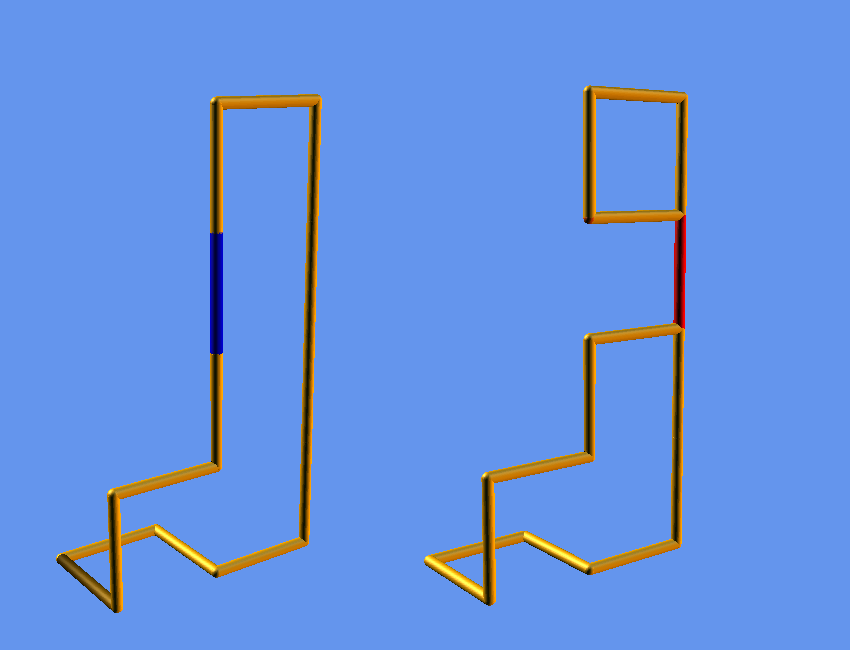
\includegraphics[width = \textwidth]{Systemmodelle/Ungueltiger_Zug.png}
	  \caption{Parallele Kantenvereinigung}
	  \label{fig:zug1}
	\end{figure}

Der Knoten auf der linken Seite \ref{fig:zug1} beschreibt eine gültige Spielsituation. Der Spieler wählt eine Kante (blaue Hervorhebung) aus, um einen weiteren Zug vorzunehmen.
Einem Spieler ist es nicht möglich, zwei parallele Kanten (hier: die Blaue und die Rote) zu einer Kante zu vereinen. Der Knoten soll immer aus einem geschlossenen Kreis von Kanten bestehen. Der Knoten auf der rechten Seite \ref{fig:zug1} ist daher eine ungültige Spielsituation.

\clearpage

	\begin{figure}[htb]
	  \centering
	  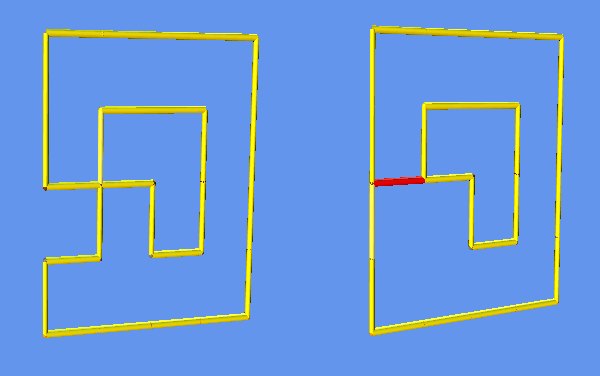
\includegraphics[width = \textwidth]{Systemmodelle/Ungueltiger_Zug2.png}
	  \caption{{\color{red}Änderung der Kantenzuordnung}}
	  \label{fig:zug2}
	\end{figure}
	
Auf der 

\clearpage

\section{Grafische Bedienuns-Oberflächen}

	\begin{figure}[ht]
	  \centering
	  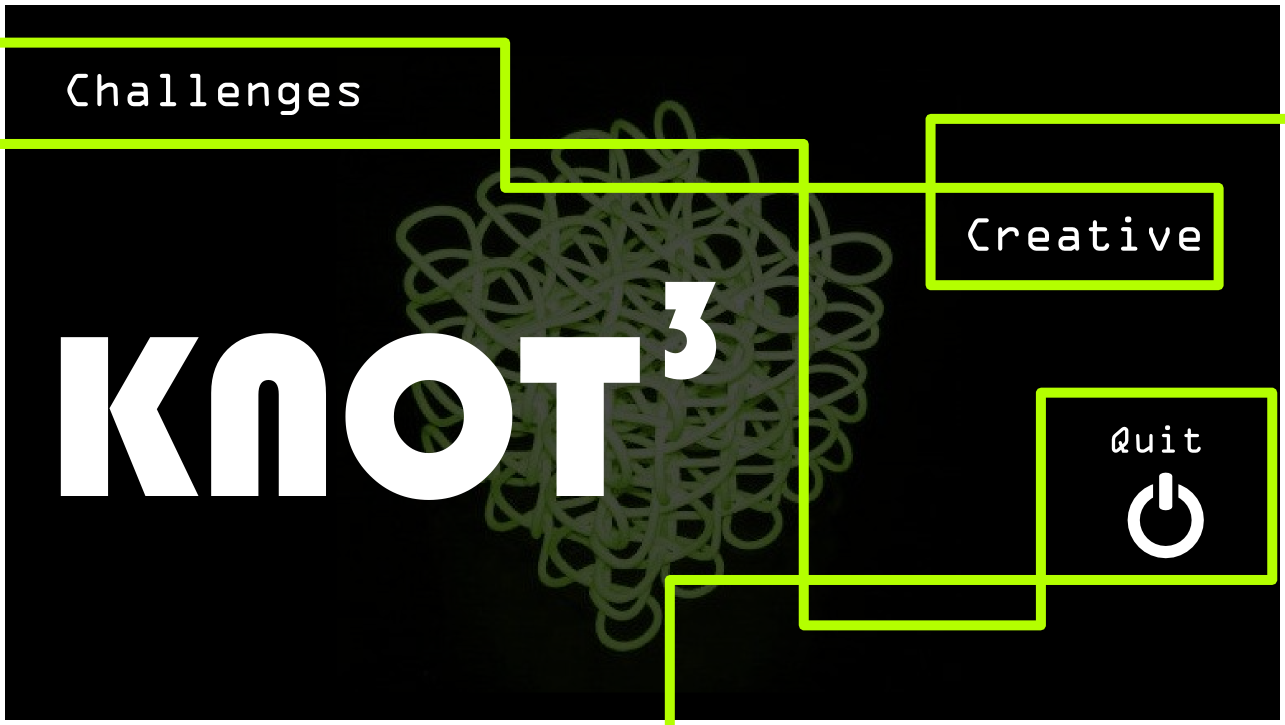
\includegraphics[width = 0.95\textwidth]{Systemmodelle/01_Knot3-mainscreen.png}
	  \caption{Hauptmenü}
	\end{figure}

	\begin{figure}[ht]
	  \centering
	  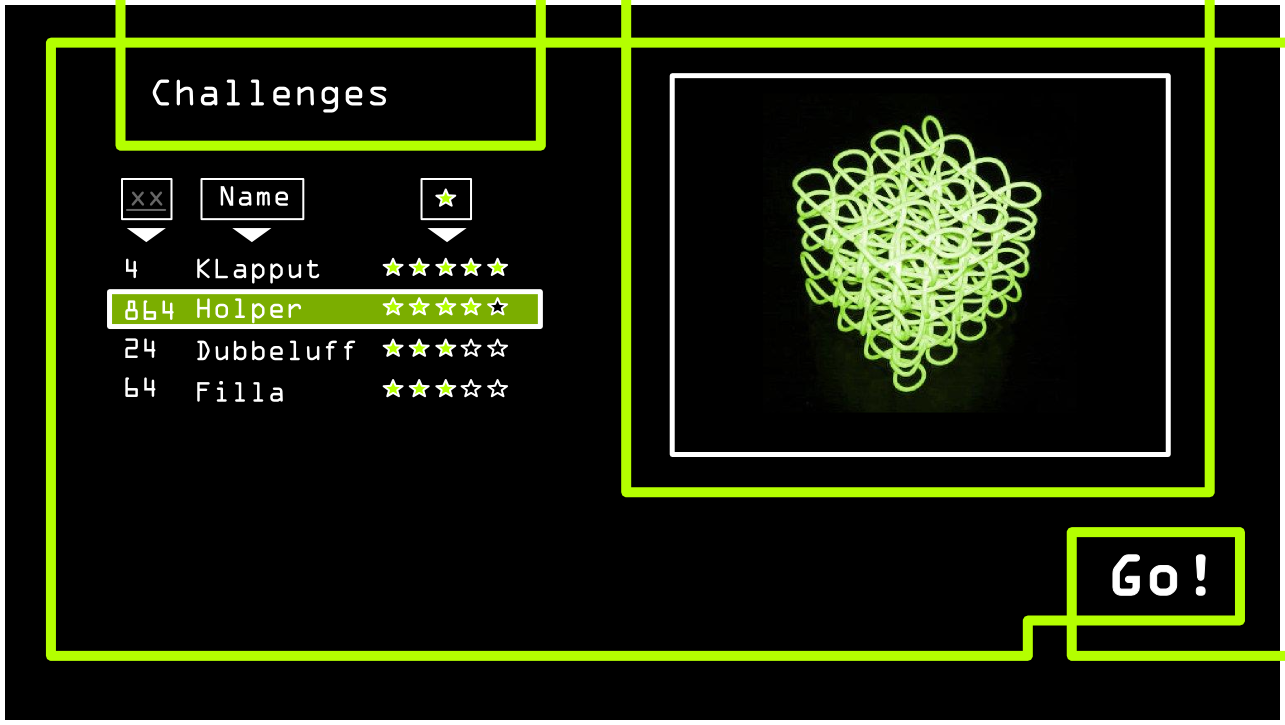
\includegraphics[width = 0.95\textwidth]{Systemmodelle/04_Knot3-select-Challenge.png}
	  \caption{Menü für Herausforderungen, mit Ausschnitt der Bestenliste}
	\end{figure}
	
	\begin{figure}[ht]
	  \centering
	  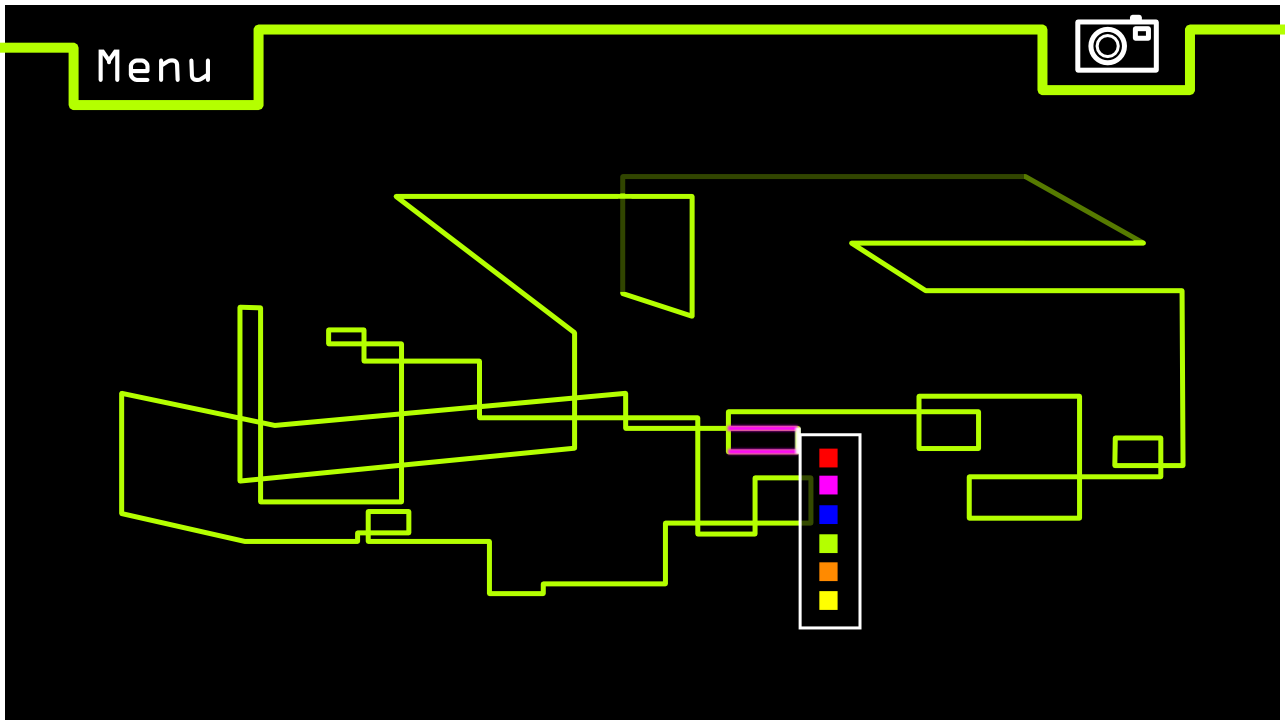
\includegraphics[width = 0.95\textwidth]{Systemmodelle/05_Knot3-Colour-select.png}
	  \caption{Creative: Kantenfärben}
	\end{figure}
	
	\begin{figure}[ht]
	  \centering
	  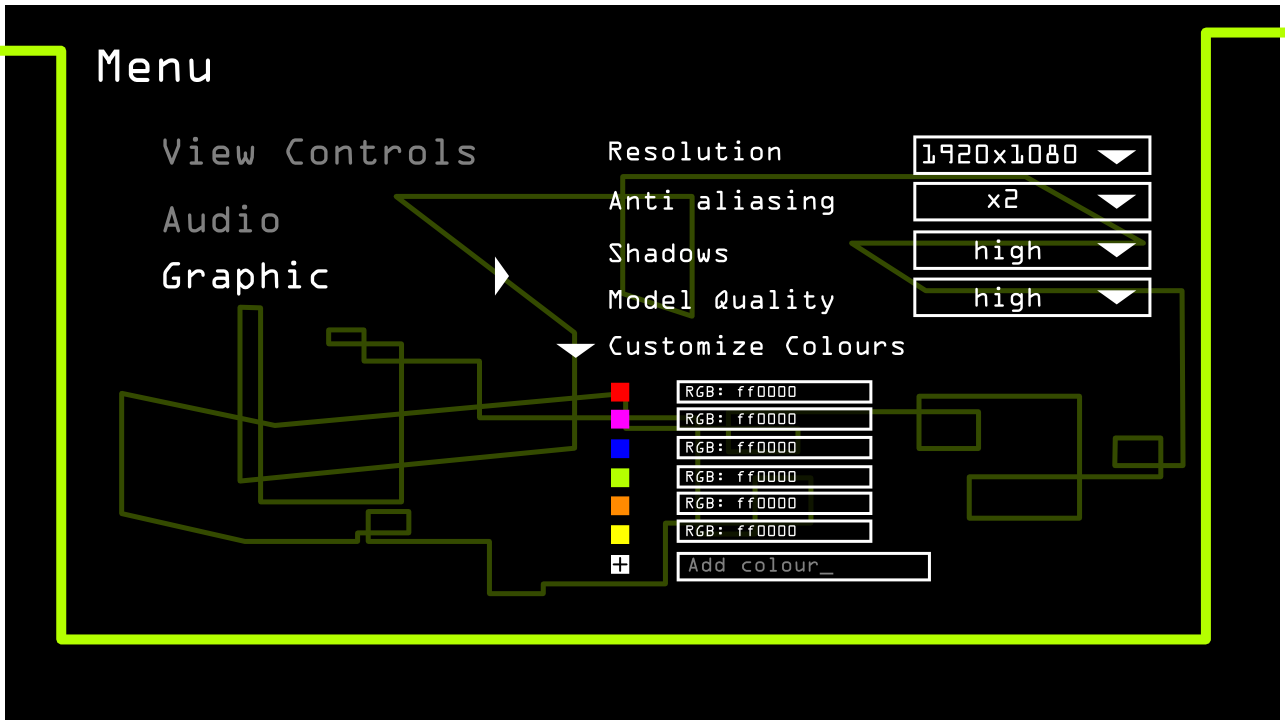
\includegraphics[width = 0.95\textwidth]{Systemmodelle/08_Knot3-menu-graphics.png}
	  \caption{Menü f. Grafikeinstellungen}
	\end{figure}

	
\clearpage
	
\section{Anwendungsfälle}

~\\
...

	\begin{figure}[ht]
	  \centering
	  \includesvg[svgpath=Systemmodelle/, width = \textwidth]{inGame}
	  \caption{Interaktionen während eines Spiels (allgemein)}
	\end{figure}

%	\begin{figure}[ht]
%	  \centering
%	  \includesvg[width = \textwidth]{Anwendungsfall}
%	  %\caption{...}
%	\end{figure}

